\documentclass[12pt,a4paper,oneside]{article}

\usepackage[utf8]{inputenc}
\usepackage[portuguese]{babel}
\usepackage[T1]{fontenc}
\usepackage{amsmath}
\usepackage{amsfonts}
\usepackage{amssymb}
\usepackage{graphicx}
\usepackage{xcolor}
\usepackage{multicol}
% Definindo novas cores
\definecolor{verde}{rgb}{0.25,0.5,0.35}

\author{\\Universidade Federal de Jataí (UFJ)\\Bacharelado em Ciência da Computação \\Linguagens Formais e Autômatos \\Esdras Lins Bispo Jr.}

\date{07 de novembro de 2019}

\title{\sc \huge Mini-Teste 4}

\begin{document}

\maketitle

{\bf ORIENTAÇÕES PARA A RESOLUÇÃO}

\small
 
\begin{itemize}
	\item A avaliação é individual, sem consulta;
	\item A pontuação máxima desta avaliação é 10,0 (dez) pontos, sendo uma das 06 (seis) componentes que formarão a média final da disciplina: quatro mini-testes (MT), uma prova final (PF) e exercícios aplicados em sala de aula pelo método de Instrução pelos Colegas (IpC);
	\item A média final ($MF$) será calculada assim como se segue
	\begin{eqnarray}
		MF & = & MIN(10, S) \nonumber \\
		S & = & [(\sum_{i=1}^{4} max(MT_i, SMT_i ) + PF].0,2  + IpC\nonumber
	\end{eqnarray}
	em que 
	\begin{itemize}
		\item $S$ é o somatório da pontuação de todas as avaliações, e
		\item $SMT_i$ é a substitutiva do mini-teste $i$.
	\end{itemize}
	\item O conteúdo exigido desta avaliação compreende o seguinte ponto apresentado no Plano de Ensino da disciplina: (3) Autômatos Finitos Não-determinísticos, (6) Gramáticas Livres-de-Contexto e (7) Autômatos com Pilha.
\end{itemize}

\begin{center}
	\fbox{\large Nome: \hspace{10cm}}
\end{center}

\newpage

\begin{enumerate}
	
	\section*{Quarto Teste}
	
	\item {\bf [Sipser 2.14]}  Converta a seguinte GLC numa GLC equivalente na forma normal de Chomsky,
	usando o procedimento apresentado em sala de aula.
	\begin{itemize}
		\item[] $A \rightarrow BAB$ | $B$ | $\epsilon$
		\item[] $B \rightarrow 00$ | $\epsilon$
	\end{itemize}
	
	\vspace*{0.3cm}
	
	{\color{blue}
		{\bf Passo 1:} Introdução de nova variável inicial.
		\begin{itemize}
			\item[] $S \rightarrow A$
			\item[] $A \rightarrow BAB$ | $B$ | $\epsilon$
			\item[] $B \rightarrow 00$ | $\epsilon$
		\end{itemize}
		
		{\bf Passo 2:} Remoção de regras $\epsilon$.
		\begin{itemize}
			\item[] $S \rightarrow A$ | $\epsilon$
			\item[] $A \rightarrow BAB$ | $B$ | $BA$ | $AB$ | $BB$
			\item[] $B \rightarrow 00$
		\end{itemize}
		
		{\bf Passo 3:} Remoção de regras unitárias.
		\begin{itemize}
			\item[] $S \rightarrow BAB$ | $00$ | $BA$ | $AB$ | $BB$ | $\epsilon$
			\item[] $A \rightarrow BAB$ | $00$ | $BA$ | $AB$ | $BB$
			\item[] $B \rightarrow 00$
		\end{itemize}
		
		{\bf Passo 4:} Inclusão de regras adicionais.
		\begin{itemize}
			\item[] $S \rightarrow CB$ | $DD$ | $BA$ | $AB$ | $BB$ | $\epsilon$
			\item[] $A \rightarrow CB$ | $DD$ | $BA$ | $AB$ | $BB$
			\item[] $B \rightarrow DD$
			\item[] $C \rightarrow BA$
			\item[] $D \rightarrow 0$
		\end{itemize}
	}
	
	\newpage
	
	\item (5,0 pt) Qual das cadeias abaixo este AP \underline{não} aceita? Justifique apropriadamente \underline{todas} as alternativas incorretas.
	
	\begin{center}
		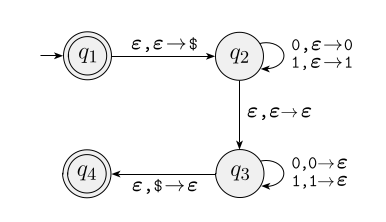
\includegraphics[width=0.5\textwidth]{images/ap3}
	\end{center}
	
	\begin{enumerate}
		\item $\epsilon$ \hspace*{0.5cm}{\color{red} {\bf Resposta: } Aceita, pois $q_1$ é estado final.}
		\item $00$
		
		\vspace*{0.3cm}
		
		{\color{red} {\bf Resposta: } Aceita. A computação de um dos ramos do AP que aceita  00 é descrita a seguir:
			\begin{enumerate}
				\item Em $q_1$, o AP empilha o $\$$ e vai para $q_2$;
				\item Em $q_2$, o AP lê 0, empilha 0, e vai para $q_3$;
				\item Em $q_3$, o AP lê 0, desempilha 0, e continua em $q_3$;
				\item Em $q_3$, o AP desempilha o $\$$, e vai para $q_4$, aceitando a cadeia.		
		\end{enumerate}}
		
		\item $11$
		
		\vspace*{0.3cm}
		
		{\color{red} {\bf Resposta: } Aceita. A computação de um dos ramos do AP que aceita  11 é descrita a seguir:
			\begin{enumerate}
				\item Em $q_1$, o AP empilha o $\$$ e vai para $q_2$;
				\item Em $q_2$, o AP lê 1, empilha 1, e vai para $q_3$;
				\item Em $q_3$, o AP lê 1, desempilha 1, e continua em $q_3$;
				\item Em $q_3$, o AP desempilha o $\$$, e vai para $q_4$, aceitando a cadeia.		
		\end{enumerate}}
		
		\item $010$ \hspace*{0.5cm} {\color{blue} {\bf Resposta: } Não aceita.}
		
	\end{enumerate}
	
\end{enumerate}

\end{document}